\documentclass[titlepage]{article}
\usepackage[pdftex]{graphicx}

% Title
\title{Lab 3: Simple DC Circuits and Resistors}
\author{Yacin Nadji}
\date{October 12th, 2006}

\begin{document}
\maketitle

\section{Statement of Objective}\label{sec:obj}
The purpose of this lab was to provide a firm basis for Ohm's Law and Kirchhoff's Law by experimenting with circuits and resistors. By comparing the theoretical results by using the theorized laws with our experimental results, we can ascertain if the laws are accurate or not.

\section{Theory}\label{sec:theory}
Ohm's Law is as follows:
\begin{equation} \label{eqn:ohms}
	V = IR
\end{equation}
Where $V$ is the potential difference of voltage across the resistor, $I$ is the current in amps through the resistor and $R$ is the resistance in ohms of the resistor. The resistors are coded by 4 colored bands that denote the amount of resistance present inside it based on this formula:
\begin{equation}
	R = A * B \times 10^C \pm D%
\end{equation}
$R$ is the resistance in ohms, $A$, $B$, $C$, and $D$ represent of the first through fourth values according to the provided color chart, respectively.\\
\\
Kirchhoff's Laws are used to determine the resistance, current and voltage of any given circuit, both series and parallel. Kirchhoff's first law states ``the current entering a junction is equal to the current leaving a junction'', Kirchhoff's second law states ``the sum of all voltage drops around a closed circuit is zero''.\\
\\
In a series circuit without any junctions, each of the resistors are identical
\[
I = I_1 = I_2 = I_3 = ... = I_n
\]
with this, and Kirchhoff's Second Law, it can be determined that
\[
	V = V_1 + V_2 + V_3 + ... + V_n
\]
By using equation (\ref{eqn:ohms}), we can ascertain:
\[
	IR = I_1R_1 + I_2R_2 + I_3R_3 + ... + I_nR_n
\]
Since the currents are equal, we can also see that:
\[
	R = R_1 + R_2 + R_3 + ... + R_n
\]
In a parallel circuit, things are a tad different considering the charges break off and go through different areas of the circuit. We begin with:
\[
	I = I_1 + I_2 + I_3 + ... + I_n
\]
With parallel circuits, the potential difference for each resistor remains the same. Therefore:
\[
	V = V_1 = V_2 = V_3 = ... = V_n
\]
and due to equation (\ref{eqn:ohms}), we get:
\begin{equation}\label{eqn:law2}
	\frac{1}{R} = \frac{1}{R_1} + \frac{1}{R_2} + \frac{1}{R_3} + ... + \frac{1}{R_n}
\end{equation}
By using these equations, we will be able to analytically approach the results we obtain experimentally with our parallel and series circuits.

\section{Equipment List}\label{sec:equipment_list}
\begin{itemize}
\item[*] Circuit Board With Resistors
\item[*] Multimeter
\item[*] DC Power Supply
\item[*] Connecting Wires
\item[*] Ammeter
\end{itemize}

\section{Procedure}\label{sec:procedure}

\subsection{Part A}\label{sub:part_a-proc}
Construct a circuit as shown in Figure 2 according to the Lab Manual. Vary the voltage on the DC Power Supply until the Voltmeter $V$ across the resistor reads 1.0 volts, then record the current using the Ammeter. Repeat these series of steps for 2.0, 3.0, 4.0, and 5.0 volts. After that, repeat the entire experiment but with a slight variation to the circuit as shown by Figure 3 in the Lab Manual.

\subsection{Part B}\label{sub:part_b-proc}

\subsubsection{Resistors in Series}\label{ssub:resistors_in_series-proc}
Construct a circuit as shown in Figure 4 of the Lab Manual using the given three resistors. Set the power supply to 10 volts, measure the current in the circuit, record this as $V_1$. Move the Voltmeter to measure the potential difference across $R_2$ and record this as $V_2$, and similarly for $R_3$. Find the total potential difference across all three resistors. Reduce the voltage supply back to zero, then switch if off. Find the resistance of each of the resistors by reading the color codes and by using an Ohmmeter as in section \ref{sub:part_a-proc}.

\subsubsection{Resistors in Parallel}\label{ssub:resistors_in_parallel-proc}
Construct the circuit as in Figure 5 of the Lab Manual using the given three resistors. Set the power supply to 10 voltes, measure $V$ and $I_1$ through $I_3$. After this, measure the total current $I$.

\subsection{Part C}\label{sub:part_c-proc}
Construct the circuit shown in Figure 6 of the Lab Manual. $R_1$ through $R_3$ are of known resistance. Using an Ammeter and a Voltmeter, find $I_1$ through $I_3$, $V$, and $V_1$ through $V_3$.

\section{Data}\label{sec:data}

\subsection{Part A}\label{sub:part_a-data}
Figure 2:
\begin{tabular}{ccc}
\hline
$V (V)$ & $I (A)$ & $R = \frac{V}{I}$\\
\hline
1 & 0.003 & 333.33\\
\hline
2 & 0.0062 & 322.58\\
\hline
3 & 0.0092 & 326.09\\
\hline
4 & 0.012 & 333.33\\
\hline
5 & 0.015 & 333.33\\
\hline
\end{tabular}
\\
\\
Figure 3:
\begin{tabular}{ccc}
\hline
$V (V)$ & $I (A)$ & $R = \frac{V}{I}$\\
\hline
1 & 0.0027 & 370.37\\
\hline
2 & 0.0052 & 384.62\\
\hline
3 & 0.008 & 375\\
\hline
4 & 0.012 & 333.33\\
\hline
5 & 0.014 & 357.14\\
\hline
\end{tabular}
\\
\\
The resistor has a resistance of $330 \pm 14$ ohms.

\subsection{Part B}\label{sub:part_b-data}

The resistors in Part B had the resistances of $1 \pm 0.05$, $5 \pm 0.25$, and $10 \pm 0.5$ ohms.

\subsubsection{Resistors in Series}\label{ssub:resistors_in_series-data}
\begin{tabular}{cc}
\hline
$I = .554 A$ & $V (V)$\\
\hline
$V_1$ & 0.594\\
\hline
$V_2$ & 3\\
\hline
$V_3$ & 5.92\\
\hline
\end{tabular}
\\
\\
The total voltage is 9.5 volts.

\subsubsection{Resistors in Parallel}\label{ssub:resistors_in_parallel-data}
\begin{tabular}{cc}
\hline
$V = 9.8 V$ & $I (A)$\\
\hline
$I_1$ & 0.0094\\
\hline
$I_2$ & 0.0019\\
\hline
$I_3$ & 0.001\\
\hline
\end{tabular}
The total current is 0.001 amps.

\subsection{Part C}\label{sub:part_c-data}
\begin{tabular}{ccc}
\hline
Element & Voltage & Current\\
\hline
Source & 10 & 1.1\\
\hline
$R_1$ & 3.6 & 1.1\\
\hline
$R_2$ & 6.39 & 0.7\\
\hline
$R_3$ & 6.39 & 0.4\\
\hline
Whole Circuit & 9.99 & 1.1\\
\hline
\end{tabular}
The total resistance through the circuit was $9120 \Omega$, calculated and measured.

\section{Analysis of Data}\label{sec:analysis_of_data}

\subsection{Part A}\label{sub:part_a-analysis}
Figure 2:\\
\\
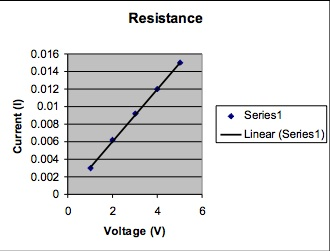
\includegraphics{1.jpg}
\\
\\
\newpage
Figure 3:\\
\\
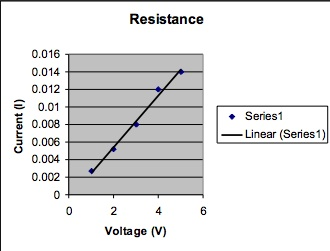
\includegraphics{2.jpg}
\\
\\
As can plainly be observed, the resistance $R$ is equal to the voltage divided by the current, $\frac{V}{I}$. With the plot of $V$ vs. $I$, the value of $R$ will be equivalent to the slope of the linear regression that best matches the data. In our case, $R = 335.4 \Omega$ and $R = 337.13 \Omega$ for the first and second experiment, respectively. Based on this, our \% error is:
\[
	\% Error = \frac{335.4 - 330}{330} * 100 = 1.6 %
\]
and
\[
	\% Error = \frac{337.13 - 330}{330} * 100 = 2.1 %
\]
As you can see, both calculations are relatively close, however, there is a discrepancy. The first one should result in a closer answer, as the circuit is significantly simpler, which allows data to be collected more accurately.
\subsection{Part B}\label{sub:part_b-analysis}
$V = V_1 + V_2 + V_3 = 0.594 + 3 + 5.92 = 9.514 V$, which is very close to the measured value. First, we must calculate the individual values for the resistors: $R_1 = \frac{0.594 V}{0.554} = 1.072 \Omega$, $R_2 = \frac{3 V}{0.554} = 5.415 \Omega$, and $R_3 = \frac{5.92 V}{0.554} = 10.685 \Omega$. The total value for the resistance was calculated to be $R_{tot} = \frac{V_1}{I} + \frac{V_1}{I} + \frac{V_1}{I} = \frac{.594 V}{.554 A} + \frac{3 V}{.554 A} + \frac{5.92 V}{.554 A} = 17.173 \Omega$ or $R_{tot} = \frac{V}{I} = \frac{9.514}{0.554} = 17.173 \Omega$. As you can see, both the total values for $R$ from analysis 2 \& 3 are the same, therefore, the sum of the resistors equals the total effective resistance. For the second part, the total value for current was determined to be $I = I_1 + I_2 + I_3 = 0.0094 + 0.0019 + 0.001 = 0.0123 A$. We can calculate our \% error for current:
\[
	\% Error = \frac{0.0123 - 0.011}{0.011} * 100 = 1.1 \%
\]
We can use the individual values for current to determine their respective resistances: $R_1 = \frac{9.8 V}{0.0094} = 1042.55$, $R_2 = \frac{9.8 V}{0.0019} = 5157.89$, and $R_3 = \frac{9.8 V}{0.001} = 9800$. Based on this, the total value for $R$ was calculated to be $R_{tot} = \frac{V}{I_{tot}} = \frac{9.8}{.0123} = 797 \Omega$. Based on the results, we can calculate our \% error as such:
\[
	\% Error = \frac{797 - 16}{16} * 100 = 4881.25 \%
\]

\subsection{Part C}\label{sub:part_c-analysis}
For Part C, we obtained the following values for resistance: $R_1 = \frac{3.6 V}{0.0011} = 3272.72 \Omega$, $R_2 = \frac{6.39 V}{0.0007} = 9128.6 \Omega$, $R_3 = \frac{6.39 V}{0.0004} = 15975 \Omega$. The sum of the currents end up being $4.8 mA$, this yields the \% error:
\[
	\% Error = \frac{4.8 - 4.75}{4.75} * 100 = 1.05 \%
\]
For the second part, using a source voltage of $10 V$ and Ohm's Law (Equation \ref{eqn:ohms}):

\[
	I_{circuit} = \frac{V_{circuit}}{R_{circuit}} = \frac{10 V}{9.12 k} = 1 mA
\]
\[
	V_{R_1} = I_{circuit} R_1 = 1 mA * 3.27 k \Omega = 3.27 V
\]
\[
	R_p = \frac{R_2 * R_3}{R_2 + R_3} = \frac{9.18 * 16.1}{9.18 + 16.1} = 5.85 k \Omega
\]
\[
	V_{R_2} = V_{R_3} = I_P R_P = 1 mA * 5.85 k \Omega = 5.85 V
\]

Using these values, we can calculate our \% error:
\[
	\% Error = \frac{5.85 - 6.39}{6.39} * 100 = 8.45 \%
\]

\section{Discussion of Results}\label{sec:discussion_of_results}
\subsection{Part A}\label{sub:part_a-discussion}
Section \ref{sub:part_a-proc} was utilized to solidify the validity of Ohm's Law (\ref{eqn:ohms}). The experimental resistance we determined using the best-fit linear regression was very close to the measure value of $R$ without significant error. This solidifies the relationship of equation (Equation \ref{eqn:ohms}). As you can see, with our very accurate values for \% error, we definitely did a good job running the experiment to help make Ohm's Law more understandable.

\subsection{Part B}\label{sub:part_b-discussion}
In Section \ref{sub:part_b-proc}, we broke down and studied parallel and series circuits, utilizing the equation (\ref{eqn:law2}) developed from Kirchhoff's Laws (see: \ref{sec:theory}). Our results were unfortunately way off for this experiment, as something must have happened during data collecting. The results seemed relatively okay during data gathering, but it's obvious there was some large margin of human error during our experimentation. When dealing with series, our results were quite accurate, landing a nice \% error of 1.1 \% for current. However, when we tried doing the same thing with parallel circuits, we had an \textit{awful} \% error of 4881.25 \%. This particular circuit was quite messy, and my only guess was my group incorrectly gathered information. An error this ridiculous could only be due to faulty equipment (which I doubt is the case considering how accurate our other results were) and human error (the likely culprit).

\subsection{Part C}\label{sub:part_c-discussion}
In Section \ref{sub:part_c-proc}, we constructed a complex circuit (Figure 6 of the Lab Manual) and values for $I_1$, $I_2$, $I_3$, $V$, $V_1$, $V_2$, and $V_3$ were collected. As in \ref{sub:part_a-proc}, we achieved very positive results, and the theoretical known values and our collected experimental values were very close. While our results weren't 100 \% accurate, they did a good job of cementing the concepts of Ohm's Law (Equation \ref{eqn:ohms}) and Kirchhoff's Laws (Section \ref{sec:theory} and Equation \ref{eqn:law2}). As you can see, our relatively low \% error value of 8.45 \% does a reasonable job upholding Kirchhoffs Laws through experimentation.

\section{Conclusions}\label{sec:conclusions}
In conclusion, save for Part B for Parallel circuits, the lab went well. Our results yielded relatively good results, and small margins of error. This solidifies the teachings of Ohm's Law and Kirchhoff's Laws in the field of Electromagnetism. 

\end{document}